\documentclass[10pt]{article}

%defines page size and margins
\usepackage{geometry}
\geometry{
    letterpaper,
    left=1in,
    right=1in,
    top=1in,
    bottom=1in,
}

%Sets spacing for entire document
\usepackage{setspace}
\singlespacing

%Package for reducing space in between list items
\usepackage{enumitem}

%Math symbols
\usepackage{gensymb}
\usepackage{siunitx}

%Image path
\usepackage{graphicx}
\graphicspath{ {/} }

%Used for adjusting images
\usepackage[export]{adjustbox}

%For floating images
\usepackage{float}

\begin{document}
\title{Laboratory One --- DC Circuits}
\date{October 6, 2017}
\author{Rishabh Shah\\ 4655 4192\\ \\ Partner: Matthew Remillard}
\maketitle
\newpage

\section*{Pre-Lab}
\begin{figure}[H]
	\centering
	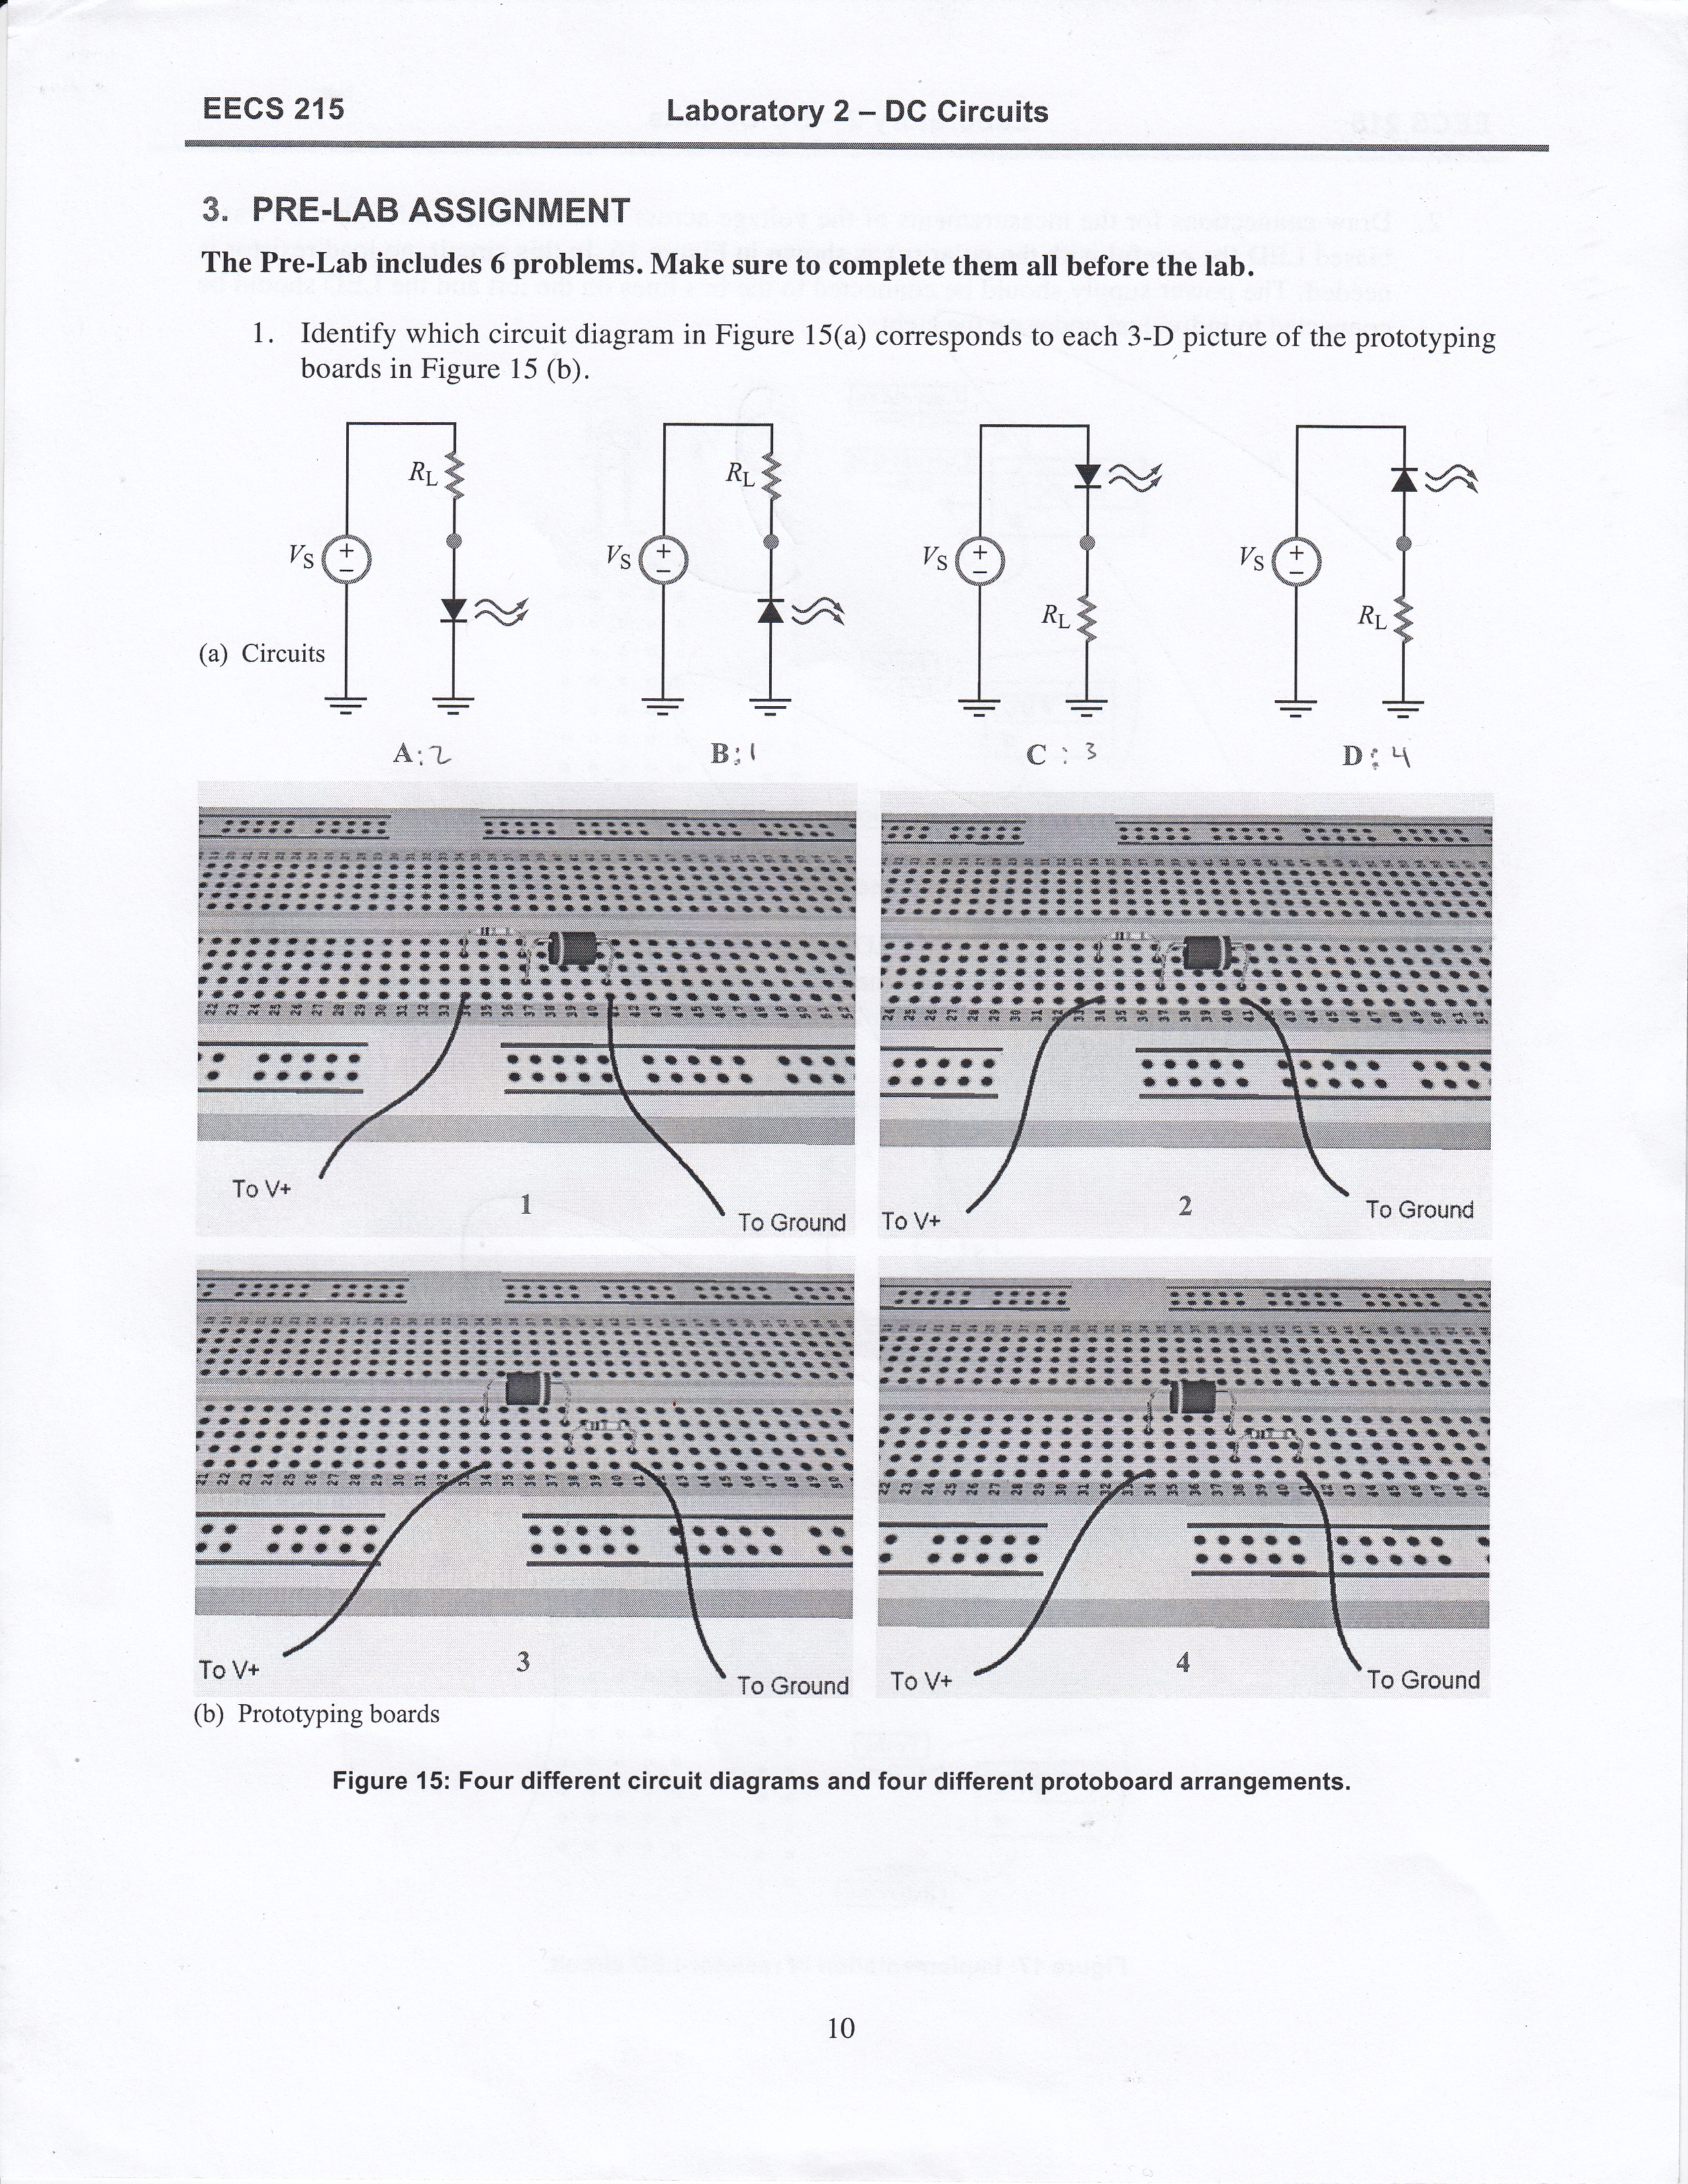
\includegraphics[width=\textwidth]{PreLabOne}
\end{figure}
\begin{figure}[H]
	\centering
	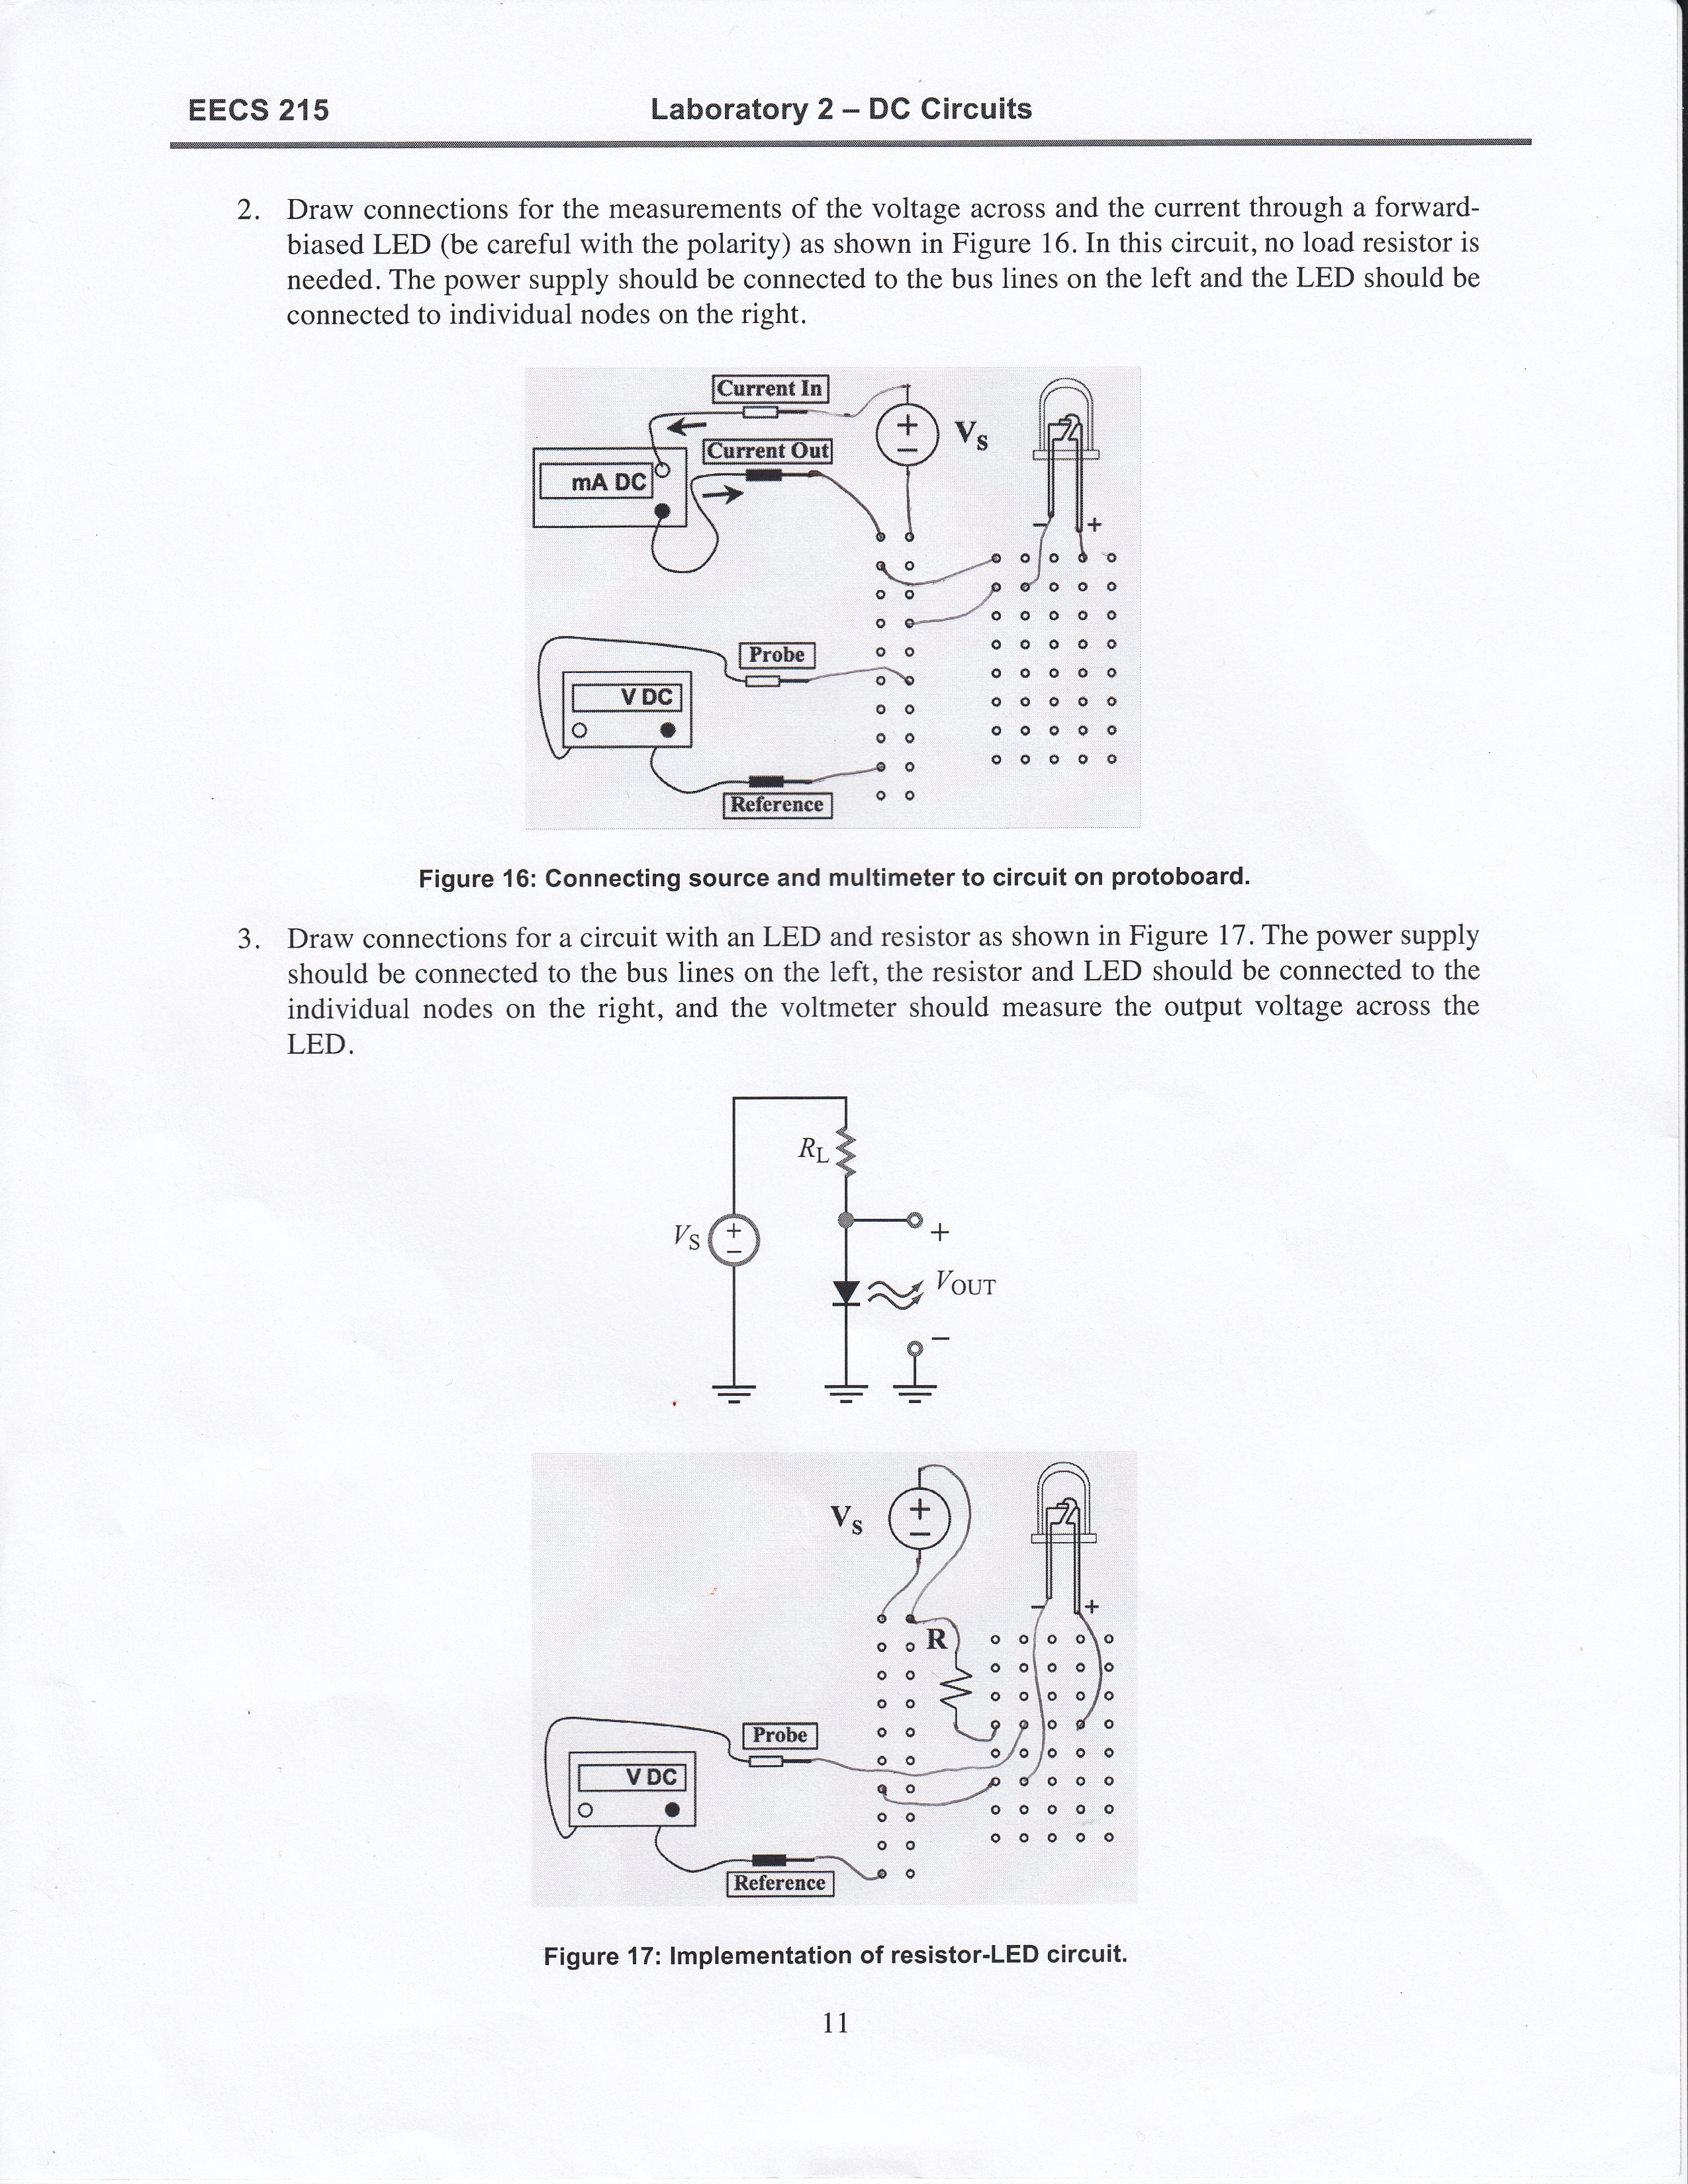
\includegraphics[width=\textwidth]{PreLabTwo}
\end{figure}
\begin{figure}[H]
	\centering
	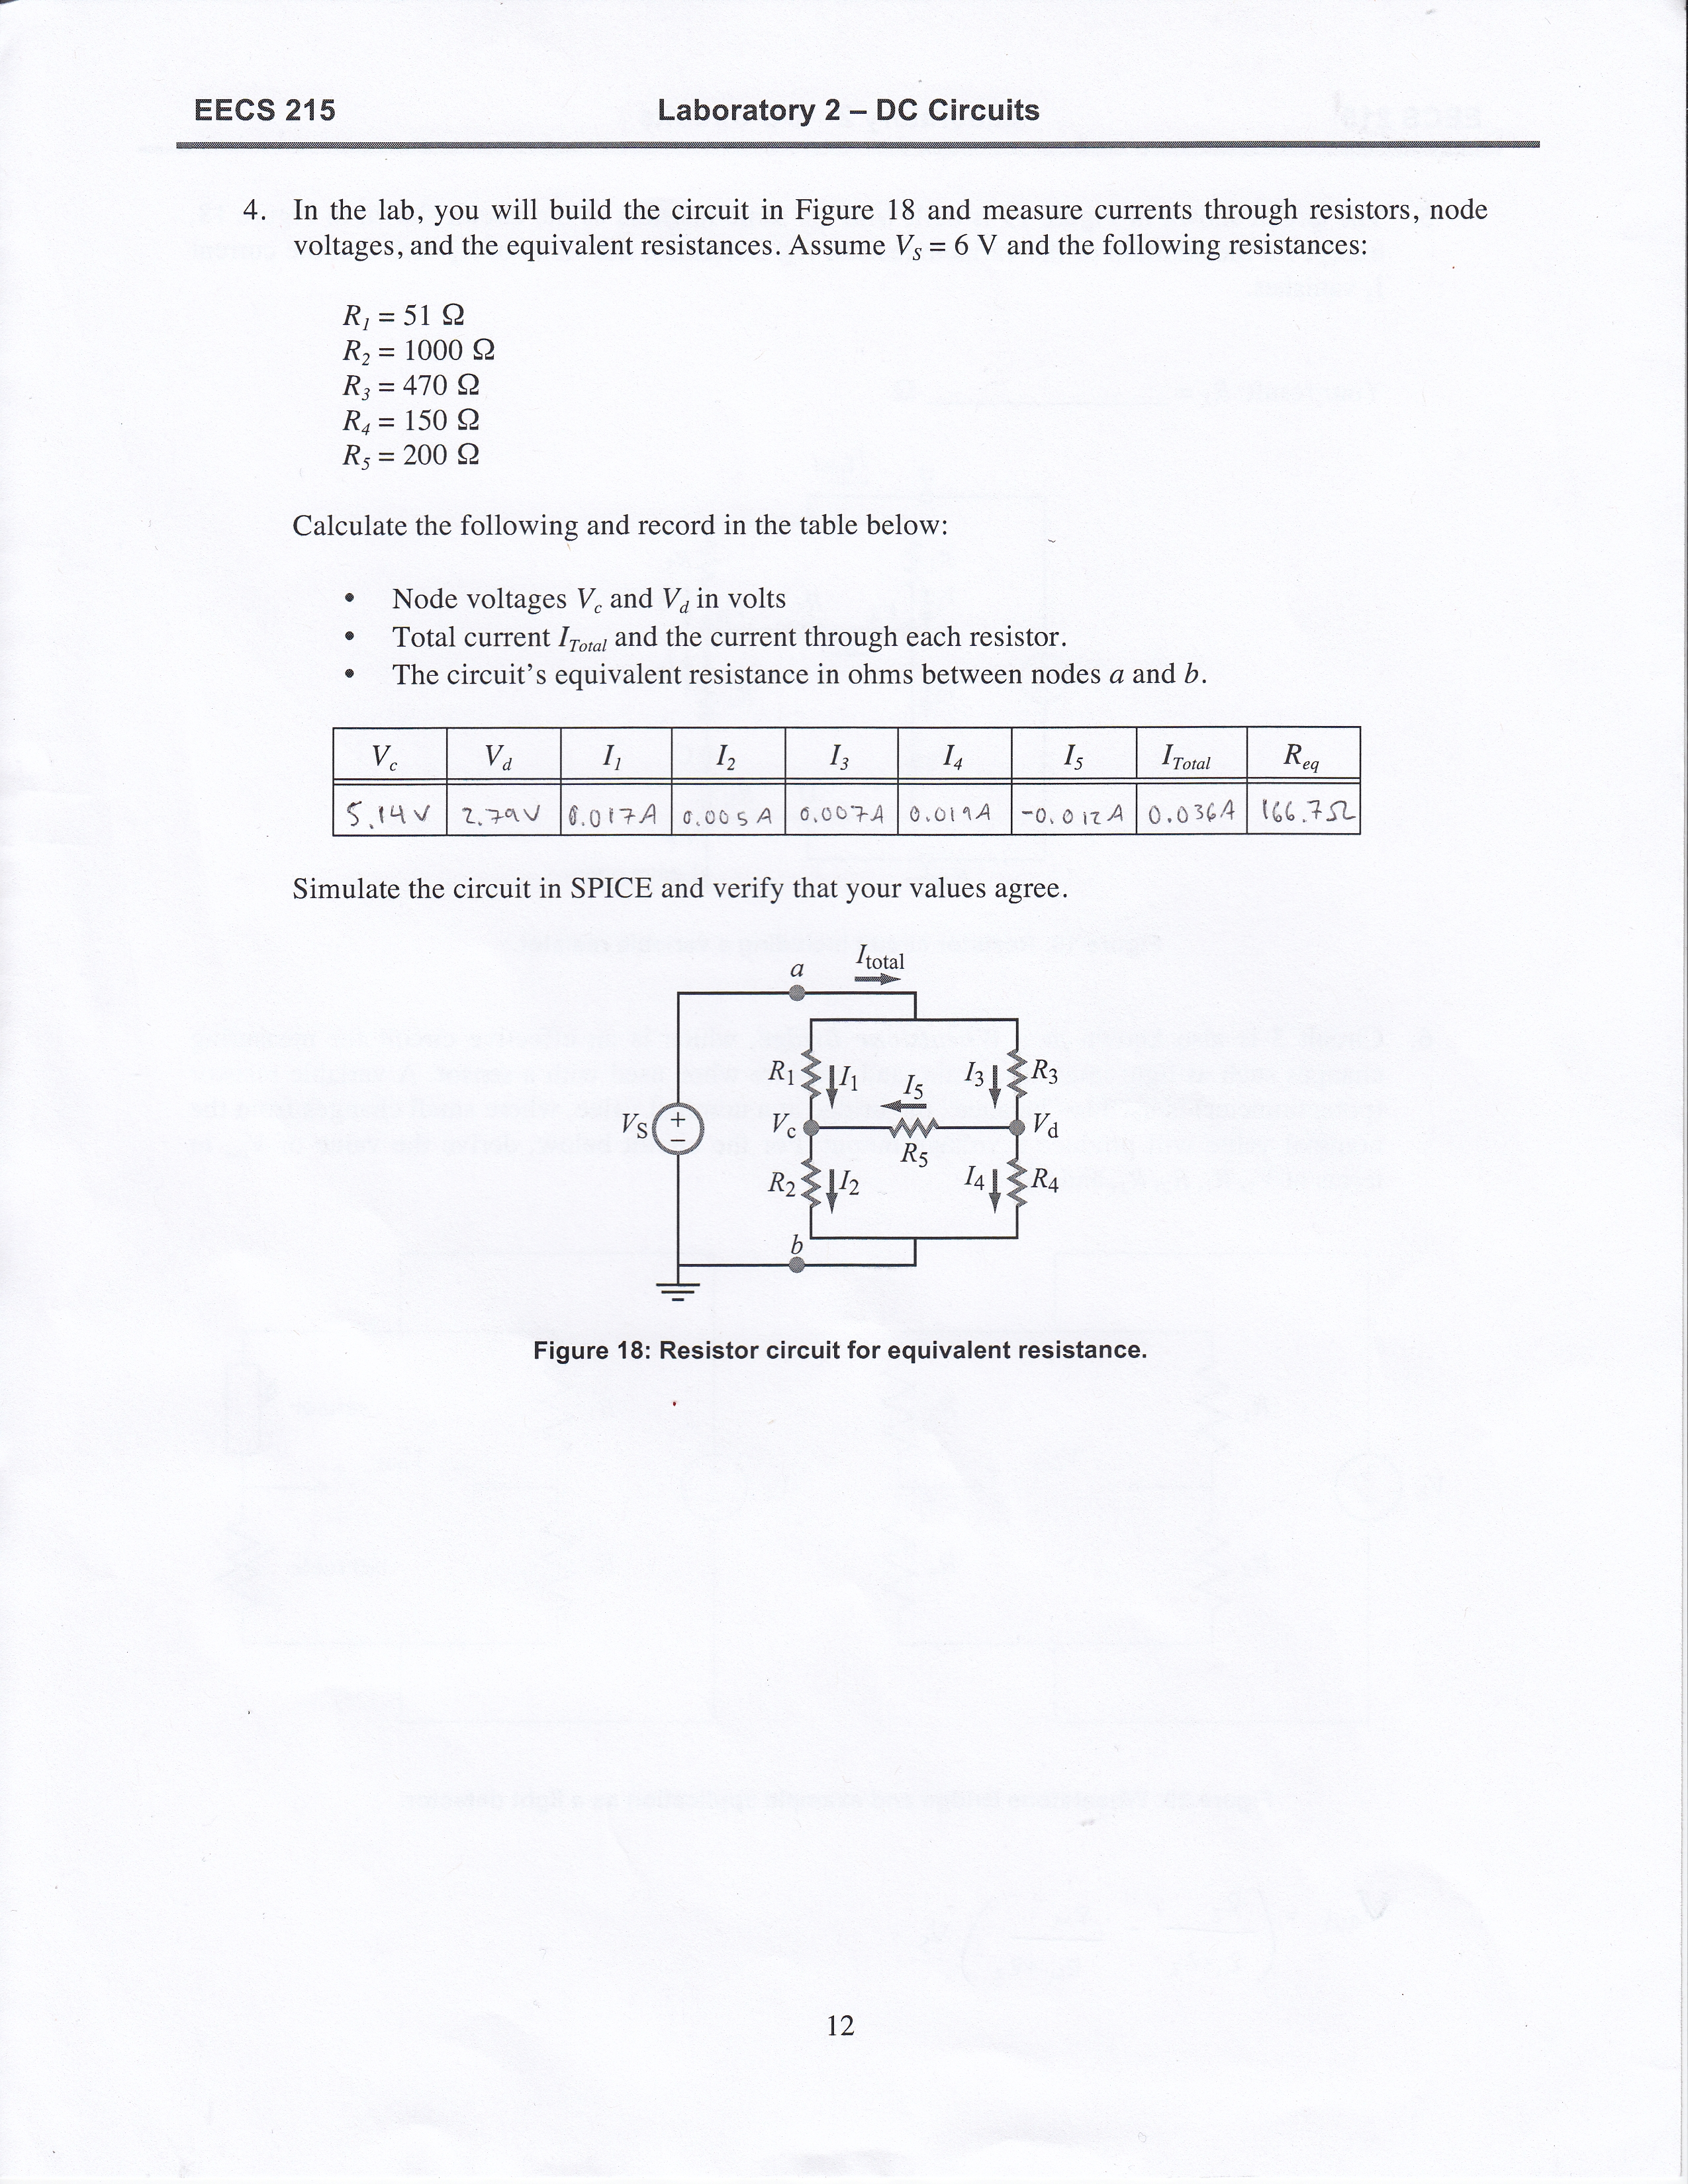
\includegraphics[width=\textwidth]{PreLabThree}
\end{figure}
\begin{figure}[H]
	\centering
	\includegraphics[width=\textwidth]{PreLabPartFour}
\end{figure}
\begin{figure}[H]
	\centering
	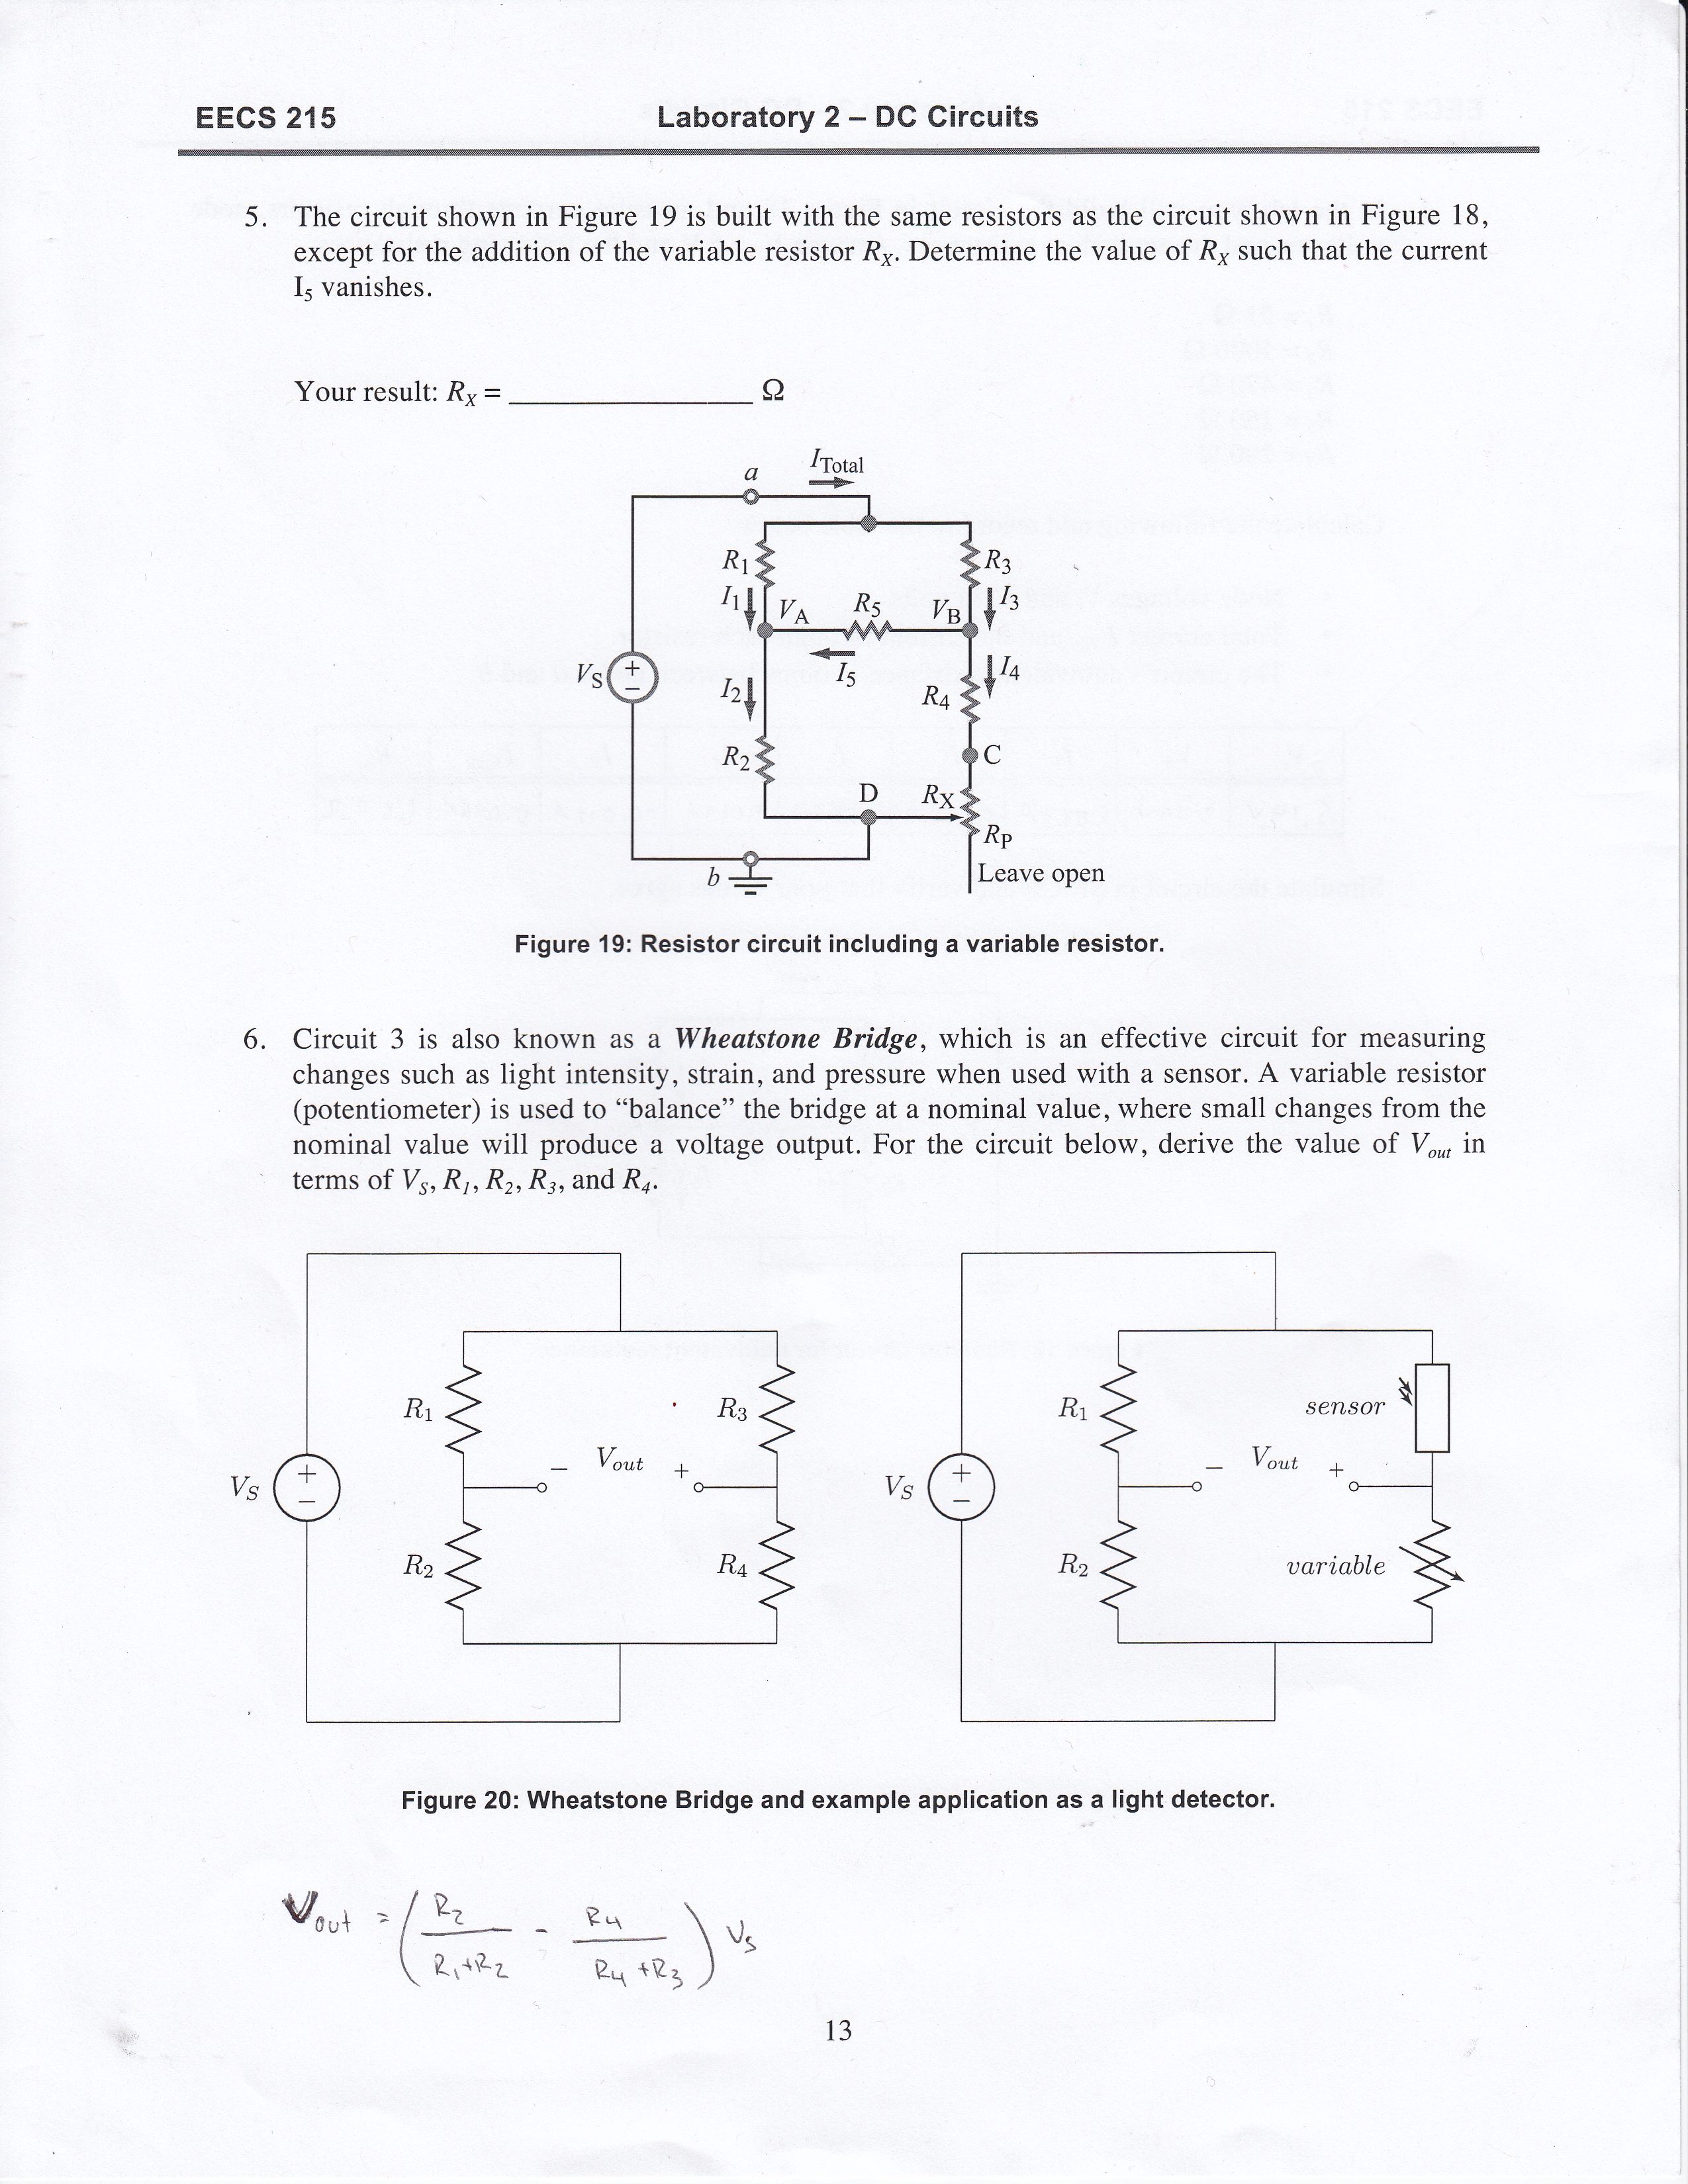
\includegraphics[width=\textwidth]{PreLabFour}
\end{figure}

\section*{Post-Lab}
\subsection*{Thevenin Equivalent}
\begin{table}[H]
	\centering
	\begin{tabular}{|c|c|c|c|c|}
		\hline
		\textbf{Component} & \textbf{Nominal Value (\si{\ohm})} & \textbf{Measure (\si{\ohm})} & \textbf{Measured \(V_L\) (V)} & \textbf{\(I_L = V_{L,meas}/R_{L,meas}\) (mA)} \\
		\hline
		\(R_S\) & 100 & 99.049 & 0 & 0 \\
		\hline
		\(R_{L1}\) & 20 & 19.784 & 1.0149 & 50.62121 \\
		\hline
		\(R_{L2}\) & 51 & 50.824 & 2.0349 & 40.03817 \\
		\hline
		\(R_{L3}\) & 100 & 97.885 & 2.9804 & 30.44797 \\
		\hline
		\(R_{L4}\) & 200 & 199.000 & 4.0036 & 20.11859 \\
		\hline
		\(R_{L5}\) & 470 & 474.040 & 4.9625 & 10.46853 \\
		\hline
		\(R_{L6}\) & 1000 & 984.600 & 5.4515 & 5.53676 \\
		\hline
	\end{tabular}
	\caption{Thevenin Equivalent circuit data}
\end{table}
\begin{figure}[H]
	\centering
	\includegraphics[width=\textwidth]{TheveninGraph}
	\caption{Graph of \(I_L\) versus \(V_L\)}
\end{figure}
\begin{figure}[H]
	\centering
	\includegraphics[width=\textwidth]{TheveninCode}
	\caption{Code used to find \(V_T\) and \(R_T\)}
\end{figure}

The calculated values for \(V_T\) and \(R_T\) are \(V_T = 60.7794V\) and \(R_T = -10.1451\Omega\). This is very different than the calculated value.

\subsection*{Light Sensor}
\subsubsection*{I}
\begin{figure}[H]
	\centering
	\includegraphics[width=\textwidth]{LSA}
	\caption{Graph of photoresistor resistance versus light intensity}
\end{figure}
\begin{figure}[H]
	\centering
	\includegraphics[width=\textwidth]{LSB}
	\caption{Graph of circuit output voltage versus light intensity}
\end{figure}
\begin{figure}[H]
	\centering
	\includegraphics[width=\textwidth]{LSC}
	\caption{Graph of circuit output voltage versus photoresistor resistance}
\end{figure}

\subsubsection*{II}
\[S = \frac{\Delta R}{\Delta lux} = \frac{7775.2-370.45}{1-1070} = -6.9268\Omega/lux\]

\[S = \frac{\Delta V_{out}}{\Delta lux} = \frac{-27.530-1.123}{1-1070} = 0.0268V/lux\]

\subsubsection*{III}
\begin{figure}[H]
	\centering
	\includegraphics[width=\textwidth]{3}
	\caption{Photoresistor circuit simulated in LTSPice}
\end{figure}

\subsubsection*{IV}
\begin{figure}[H]
	\centering
	\includegraphics[width=\textwidth]{4}
	\caption{Simulated graph of circuit output voltage versus photoresistor resistance}
\end{figure}
\begin{figure}[H]
	\centering
	\includegraphics[width=\textwidth]{LSC}
	\caption{Graph of circuit output voltage versus photoresistor resistance}
\end{figure}

When comparing the measured data to the simulated data, it looks like the slope of the graph is opposite. This is due to the voltmeter having the reversed polarity when measuring. Disregarding the reversed polarity, the two graphs are fairly similar.

\subsubsection*{V}
The sensitivity of our circuit is fairly high, as we have a sensitivity of 6 \si{\ohm} per lux. This means that for every increase in lux, the resistance of the photoresistor increases by 6 \si{\ohm}. The circuit is fairly linear, as shown by the graphs in Part I. The accuracy of the circuit is also fairly high due to the similarities between the simulated graph and the measured data, including the slope of both graphs.

\subsubsection*{VI}
An application of our circuit is on a solar tracking device. In such a device, photoresistors are used to compare the amount of light on all sides of a solar panel. Then the output voltages are compared, and the side with the highest amount of light is the direction in which the solar panel will be moved. This results in maximum electrical output for the solar panel. The sensitivity of the photoresistor circuits is fairly important, especially if the device is tracking at a high rate. This results in the light variation per side being much lower than if the device is tracking at a low rate. The accuracy of the photoresistor is also important, as noisy data will result in the device incorrectly tracking. The linearity of the photoresistors is not important, as the values are compared, rather than used individually.

\end{document}